\section{Theorie}
\label{sec:Theorie}
Auf eine Kugel, welche sich in einer Flüssigkeit unter Einfluss der Gravitation bewegt, wirkt die Stokessche Reibungskraft
\begin{equation}
    F_{\symup{R}}=6\symup{\pi}\eta v r.
\end{equation}
Hierbei bezeichnet $v$ die Geschwindigkeit der Kugel, $r$ den Radius selber Kugel und $\eta$ die dynamische Viskosität.
Neben der Stokesschen Reibungskraft $F_{\symup{R}}$ wirkt auch eine Auftriebskraft $F_{\symup{A}}$ und die Schwerkraft $F_{\symup{G}}$.
Fällt eine Kugel in einer viskosen Flüssigkeit stellt sich nach kurzer Zeit ein Kräftegleichgewicht ein, sodass sich die Kugel 
mit konstanter Geschwindigkeit $v$ bewegt.

Dies kann in einem Höppler-Viskosimeter untersucht werden.
\begin{figure}
    \centering
    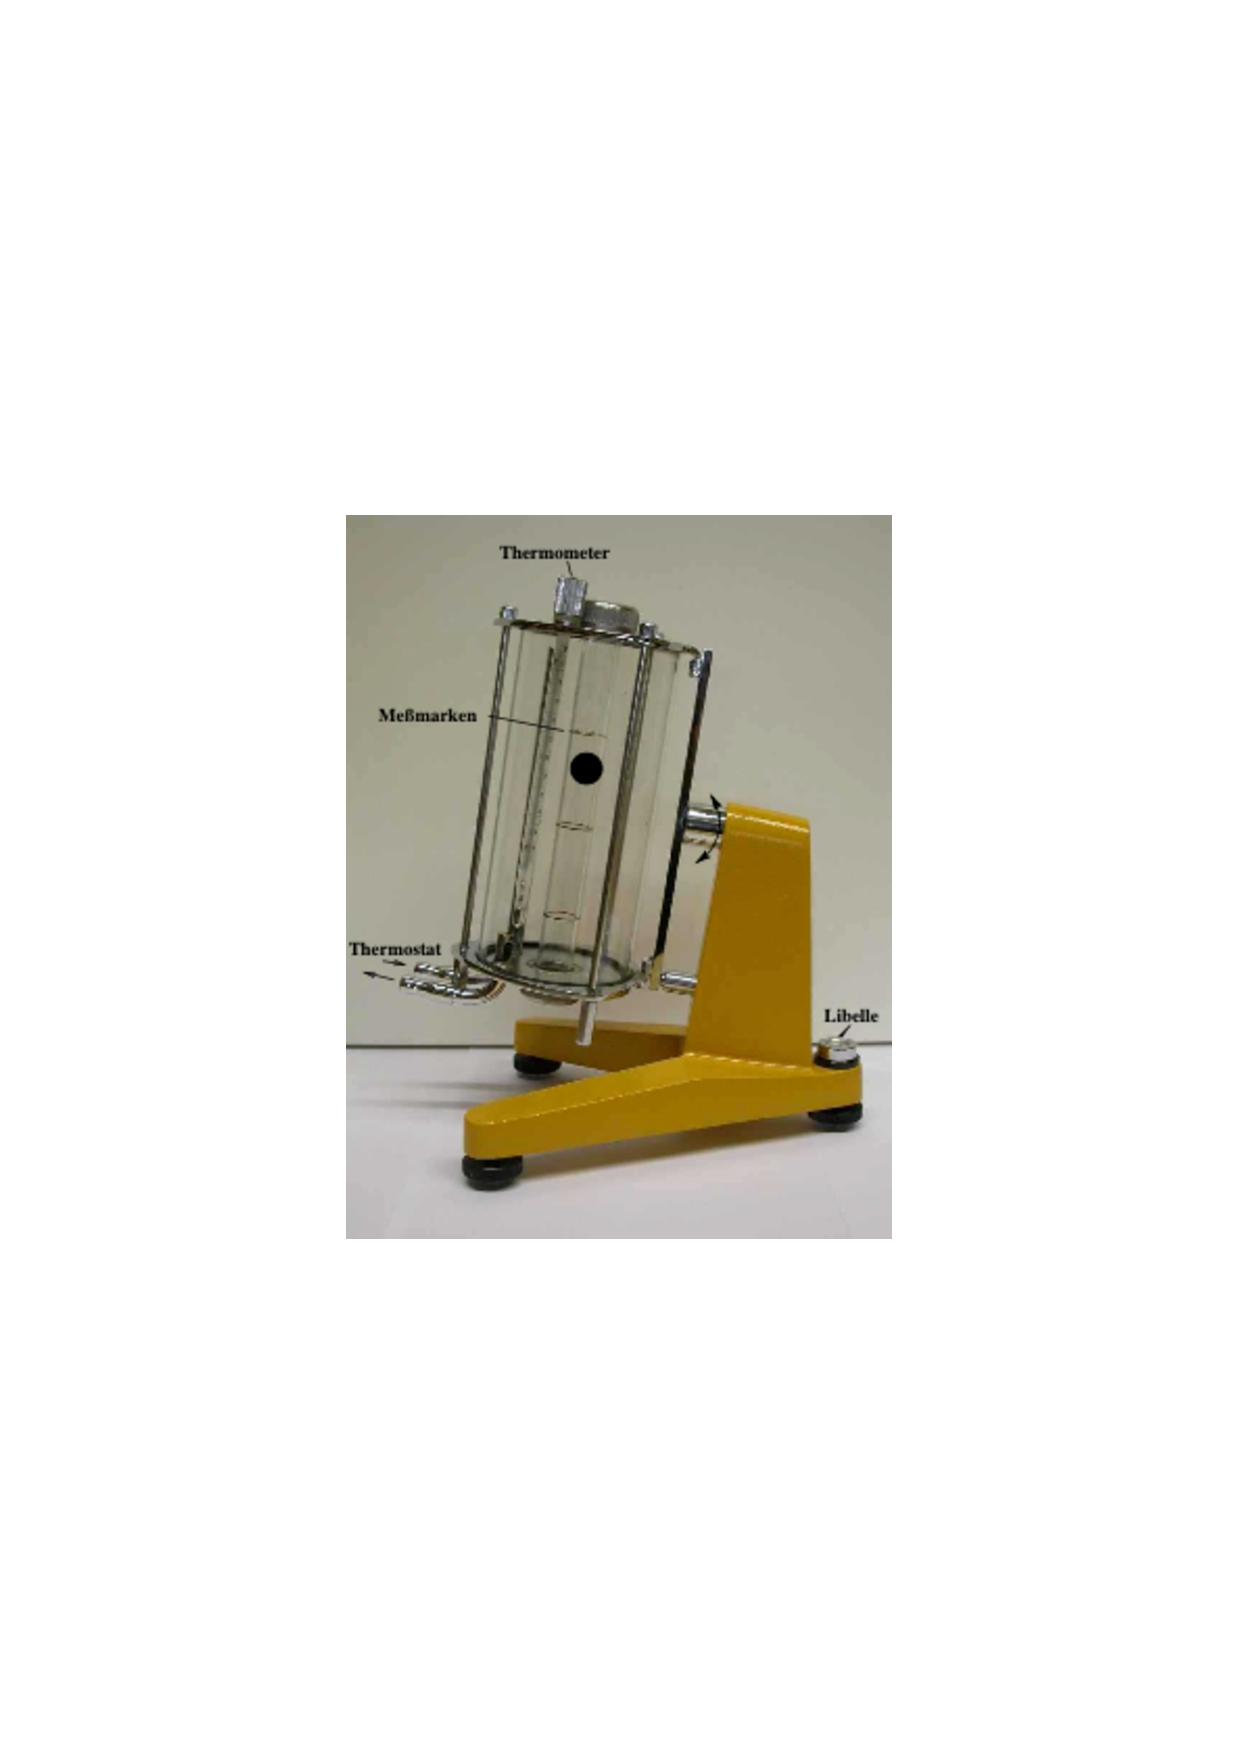
\includegraphics{content/Hoeppler-Viskosimeter.pdf}
    \caption{Ein Höppler-Viskosimeter mit regelbarer Wassertemperatur $T$ und Messmarken in einem Abstand %
     von jeweils $\Delta s = 5\unit{\centi\metre}$. \cite{v107}}
     \label{fig:Hoeppler-Viskosimeter}
\end{figure}

In diesem Versuch gilt es zu zeigen, dass die dynamische Viskosität einer Flüssigkeit von der Temperatur abhängig ist. 
Dabei ist zu beachten, dass sich ein solcher Zusammenhang nur für laminare
und nicht für turbulente Strömungen in geschlossener Form schreiben lässt. Ein Maß für die Turbulenz einer Rohrströmung ist die Reynoldszahl
\begin{equation}
    Re=\frac{\rho v_{\symup{S}}r}{\eta}.
    \label{eqn:Reynoldszahl}
\end{equation}
Die Reynoldszahl ist abhängig von der Dichte der Flüssigkeit $\rho$, der Strömungsgeschwindigkeit $v_{\symup{S}}$, dem 
Rohrdurchmessers $r$, sowie der dynamischen Viskosität $\eta$. Liegt die Reynoldszahl unter einem kritischen Wert von
$R_{\symup{crit}}\approx 1200$ \cite[341/B102]{czichos} liegt eine laminare Strömung vor.

Wenn dies erfüllt ist, lässt sich die dynamische Viskosität $\eta$ über die Formel
\begin{equation}
    \eta = K(\rho_{\symup{K}}-\rho_{\symup{Fl}})\cdot t
    \label{eqn:Viskosität}
\end{equation}
beschreiben. $K$ ist eine Apperaturkonstante und enthält die Fallhöhe von $\Delta s=10\unit{\centi\metre}$. Außerdem
bestehen auch Abhänigkeiten von der Fallzeit $t$, der Dichte der Flüssigkeit $\rho_{\symup{Fl}}$ und der Kugeldichte
$\rho_{\symup{K}}$.

Aufgrund der Temperaturabhängigkeit der Dichten, ist die dynamische Viskosität gleichermaßen temperaturabhängig und kann über 
die \textit{Andradesche Gleichung}
\begin{equation}
    \eta (T)=A\cdot e^{\frac{B}{T}}
    \label{eqn:Andradesche Gleichung}
\end{equation}
beschrieben werden.

% \subsection{Viskosität}
% \label{sec:Viskosität}

% \subsection{Reynoldszahl}
% \label{sec:Reynoldszahl}

% \subsection{Das Höppler-Viskosimeter}
% \label{sec:Das Höppler-Viskosimeter}